% ---------------------------------------------------------------------
% 2.11 Métricas de evaluación
% ---------------------------------------------------------------------
\section[MÉTRICAS DE EVALUACIÓN]{Métricas de evaluación}
\label{sec:metricas}

El desempeño de un sistema basado en la P300 puede evaluarse en dos niveles: el de la
clasificación de cada época como objetivo o no objetivo, que mide la calidad del modelo de
aprendizaje profundo, y el del sistema completo, que mide qué tan rápido y con qué exactitud el
usuario logra seleccionar caracteres.

\subsection{Matriz de confusión}

En un problema de clasificación binaria, las predicciones del modelo pueden compararse con las
etiquetas reales mediante una tabla cruzada conocida como matriz de confusión, representada en la
Figura~\ref{fig:confusion}. Sus cuatro celdas corresponden a los verdaderos positivos (TP), épocas
con P300 clasificadas correctamente; los falsos positivos (FP), épocas sin P300 clasificadas como
positivas; los verdaderos negativos (TN), épocas sin P300 clasificadas correctamente; y los falsos
negativos (FN), épocas con P300 que el modelo no detectó \cite{fawcett2006}.

\begin{figure}[htbp]
\centering
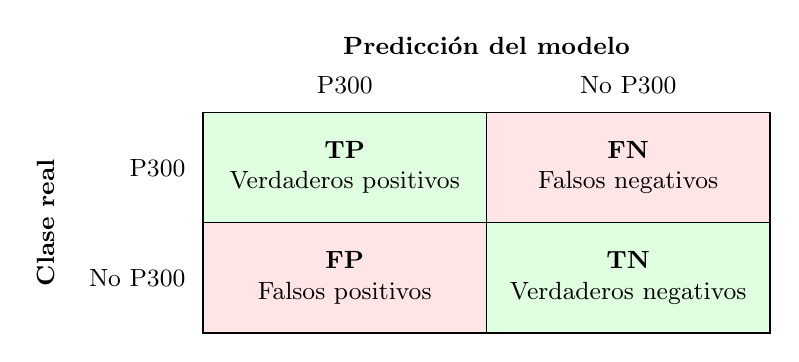
\begin{tikzpicture}[celda/.style={draw, minimum width=3.6cm, minimum height=1.4cm, align=center, font=\small}]
  \node[celda, fill=green!12] (tp) at (0,0) {\textbf{TP}\\Verdaderos positivos};
  \node[celda, fill=red!10] (fn) at (3.6,0) {\textbf{FN}\\Falsos negativos};
  \node[celda, fill=red!10] (fp) at (0,-1.4) {\textbf{FP}\\Falsos positivos};
  \node[celda, fill=green!12] (tn) at (3.6,-1.4) {\textbf{TN}\\Verdaderos negativos};
  \node[font=\small] at (0,1.05) {P300};
  \node[font=\small] at (3.6,1.05) {No P300};
  \node[font=\small\bfseries] at (1.8,1.55) {Predicción del modelo};
  \node[font=\small, anchor=east] at (-1.9,0) {P300};
  \node[font=\small, anchor=east] at (-1.9,-1.4) {No P300};
  \node[font=\small\bfseries, rotate=90] at (-3.8,-0.7) {Clase real};
\end{tikzpicture}
\caption{Matriz de confusión para la clasificación binaria de épocas. Elaboración propia.}
\label{fig:confusion}
\end{figure}

\subsection{Métricas de clasificación}

A partir de estos cuatro valores se calculan las métricas que se presentan en la
Tabla~\ref{tab:metricas}. La exactitud mide el porcentaje total de aciertos, pero como se discutió
en la Sección~\ref{sec:speller}, en un conjunto con una proporción de 1 a 5 entre clases puede
resultar engañosa, por lo que conviene complementarla con la sensibilidad, que indica qué
proporción de las épocas con P300 fueron detectadas, la precisión, que indica qué proporción de las
detecciones fueron correctas, y el F1-score, que es la media armónica de ambas
\cite{fawcett2006}. La exactitud balanceada, que promedia la sensibilidad y la especificidad, es
otra alternativa que no se ve afectada por el desbalance.

\begin{table}[htbp]
\centering
\caption{Métricas de evaluación para la clasificación binaria}
\label{tab:metricas}
\small
\begin{tabularx}{\textwidth}{L{2.8cm}YL{4.4cm}}
\toprule
\textbf{Métrica} & \textbf{Descripción} & \textbf{Fórmula} \\
\midrule
Exactitud (\textit{accuracy}) & Proporción de predicciones correctas sobre el total. & $\dfrac{TP+TN}{TP+TN+FP+FN}$ \\[10pt]
Precisión (\textit{precision}) & Proporción de épocas clasificadas como P300 que realmente lo son. & $\dfrac{TP}{TP+FP}$ \\[10pt]
Sensibilidad (\textit{recall}, TPR) & Proporción de épocas con P300 que fueron detectadas. & $\dfrac{TP}{TP+FN}$ \\[10pt]
Especificidad (TNR) & Proporción de épocas sin P300 clasificadas correctamente. & $\dfrac{TN}{TN+FP}$ \\[10pt]
Tasa de falsos positivos (FPR) & Proporción de épocas sin P300 clasificadas como positivas. & $\dfrac{FP}{FP+TN} = 1-\text{TNR}$ \\[10pt]
F1-score & Media armónica entre precisión y sensibilidad. & $2\cdot\dfrac{\text{Precisión}\cdot\text{Sensibilidad}}{\text{Precisión}+\text{Sensibilidad}}$ \\[10pt]
Exactitud balanceada & Promedio de la sensibilidad y la especificidad. & $\dfrac{\text{TPR}+\text{TNR}}{2}$ \\
\bottomrule
\end{tabularx}
\par\smallskip{\footnotesize Elaboración propia con información de \cite{fawcett2006}.}
\end{table}

\subsection{Curva ROC y área bajo la curva}

Los clasificadores de la P300 suelen producir un puntaje continuo, y la etiqueta final depende del
umbral que se elija: al disminuirlo se detectan más épocas con P300, pero también aumentan los
falsos positivos. La curva ROC (\textit{Receiver Operating Characteristic}) representa este
compromiso graficando la sensibilidad contra la tasa de falsos positivos para todos los umbrales
posibles, y el área bajo esta curva (AUC) resume el desempeño en un solo número que puede
interpretarse como la probabilidad de que el clasificador asigne un puntaje mayor a una época
positiva elegida al azar que a una negativa elegida al azar \cite{fawcett2006}. Un AUC de 0.5
corresponde a un clasificador aleatorio, cuyas distribuciones de puntajes para ambas clases se
encuentran superpuestas, mientras que un AUC de 1 indica una separación perfecta, como se ilustra
en la Figura~\ref{fig:roc}; esta es la métrica utilizada en los trabajos de Alvarado-González et al.
y de Contreras, en el que se considera aceptable a partir de 0.7 \cite{alvarado2021,contreras2021}.

\begin{figure}[htbp]
\centering

\includegraphics[width=\textwidth]{02-marco-referencial/roc_auc.pdf}
\caption{(a) Distribuciones de puntajes de un clasificador para ambas clases y un umbral de
decisión. (b) Curvas ROC para distintos grados de separación entre clases. Elaboración propia.}
\label{fig:roc}
\end{figure}

\subsection{Métricas a nivel de sistema}

Una alta AUC en la clasificación de épocas no garantiza por sí sola una comunicación eficiente,
pues la velocidad depende también del número de repeticiones necesarias para seleccionar cada
carácter. Por ello, en los sistemas de deletreo se reporta la exactitud por carácter en función
del número de repeticiones, los caracteres por minuto y la tasa de transferencia de información
(ITR), que de acuerdo con Wolpaw et al. se calcula en bits por selección como
\cite{wolpaw2000,wolpaw2002}
\begin{equation}
B = \log_2 N + P\log_2 P + (1-P)\log_2\!\left(\frac{1-P}{N-1}\right),
\label{eq:itr}
\end{equation}
donde $N$ es el número de opciones posibles, 36 en una matriz de $6\times6$, y $P$ es la exactitud
por carácter; al multiplicar $B$ por el número de selecciones por minuto se obtiene la ITR en bits
por minuto. La Figura~\ref{fig:itr} muestra que, para una misma exactitud, reducir el número de
repeticiones incrementa notablemente la ITR, aunque en la práctica disminuir las repeticiones
también reduce la exactitud, por lo que el número óptimo de repeticiones es aquel que maximiza el
producto de ambos efectos.

\begin{figure}[htbp]
\centering

\includegraphics[width=\textwidth]{02-marco-referencial/itr_repeticiones.pdf}
\caption{(a) Bits por selección en función de la exactitud para $N=36$ según la
Ecuación~\eqref{eq:itr}. (b) ITR teórica en función del número de repeticiones para tres niveles
de exactitud, considerando 175~ms por intensificación y 2.5~s entre caracteres. Elaboración
propia.}
\label{fig:itr}
\end{figure}
